
%version 2: \usepackage{hyperref}


%%%%%%%%%%%%%%%%%%%%%%%%%%%%%%%%%%%%%%%%%%%%%%%%%%%%%%%%%%%%%%%%%%%%%%%%
%Para las ecuaciones siempre es Ec.(n).
%Para las figuras siempre es Fig.n, incluso en el caption de la figura. Tambien las Tablas
%Para las referencias es [n]
%%%%%%%%%%%%%%%%%%%%%%%%%%%%%%%%%%%%%%%%%%%%%%%%%%%%%%%%%%%%%%%%%%%%%%%%

\documentclass[
reprint,
%notitlepage,
%superscriptaddress,
%groupedaddress,
%unsortedaddress,
%runinaddress,
%frontmatterverbose, 
%preprint,
%showpacs,preprintnumbers,
%nofootinbib,
%nobibnotes,
%bibnotes,
%11 pt,
amsmath,
amssymb,
%aps,
%pra,
prb,
%rmp,
%tightenlines %esto hizo el milagro de sacar los espacios en blancos estocásticos (?)
%prstab,
%prstper,
%floatfix,\textbf{}
]{revtex4-1} %Instalar primero para usarlo. Paquete malo.

%\documentclass[onecolumn, aps, amsmath,amssymb ]{article}
\usepackage{lipsum}  
\usepackage{graphicx}% Include figure files
\usepackage{subfig}
\usepackage{braket}
\usepackage{comment} %comment large chunks of text
\usepackage{dcolumn}% Align table columns on decimal point
\usepackage{bm}% bold math
%\usepackage{hyperref}% add hypertext capabilities
\usepackage[mathlines]{lineno}% Enable numbering of text and display math
%\linenumbers\relax % Commence numbering lines
\usepackage{mathtools} %% Para el supraíndice

\usepackage[nice]{nicefrac}

%%%%%%%El Señor Español%%%%%%%%%%%%%%%%%%%%%%%%%%%
\usepackage[utf8]{inputenc} %acento
\usepackage[
spanish, %El lenguaje.
es-tabla, %La tabla y no cuadro.
activeacute, %El acento.
es-nodecimaldot %Punto y no coma con separador de números
]{babel}
\usepackage{microtype} %para hacerlo más bonito :33 como vos (?) 
%%%%%%%%%%%%%%%%%%%%%%%%%%%%%%%%%%%%%%%%%%%%%%%%%%%
%%%%%%%%% Para que las imágenes se queden dónde las quiero (?
\usepackage{float}
%%%%%%%%%%
\usepackage{enumitem}
\usepackage{hyperref} % Para usar \url

%%%%%%%%Cambia a Fig de Figure%%%%%%%%%%
\makeatletter
\renewcommand{\fnum@figure}{Fig. \thefigure} 
\makeatother
%%%%%%%%%%%%%%%%%%%%%%%%%%%%%%%%%%%%%%%%
\raggedbottom



   %\usepackage[caption=false]{subcaption}

\begin{document}
%%%%%%%%%%%%%%%%%%%%%%%%%%%%%%%%%%Título%%%%%%%%%%%%%%%%%%%%%%%%%%%%%%%%%%%%%%
%%%%%%%%%%%%%%%%%%%%%%%%%%%%%%%%%%%%%%%%%%%%%%%%%%%%%%%%%%%%%%%%%%%%%%%%%%%%%%

\title{Práctica 0: Introducción a Python, Numpy, Matplotlib y Scipy.}
\author{Evelyn~G.~Coronel}

\affiliation{
Aprendizaje Profundo y Redes Neuronales Artificiales\\ Instituto Balseiro\\}

\date[]{\lowercase{\today}} %%lw para lw, [] sin date


\maketitle
%\onecolumngrid


\section*{Ejercicio 1}

Para este ejercicio se utiliza la librería \verb|numpy.linealg|. Se inicializa una matriz $A$ de los coeficientes de las ecuaciones, así como también el vector $b$ para trabajar con $A\cdot x = b $.



Para solucionar este sistema de ecuaciones, se utiliza la expresión $x=A^{-1}b$. Primero debe verificarse la existencia de una solución única, para esto calculamos el determinante de $A$. Si la matriz $A$ no es invertible, entonces  $\det(A)=0$, por lo que el programa termina ahí. Caso contrario, se usa la función 

\verb|x= np.linalg.solve(A, b)|

\section*{Ejercicio 2}

En este ejercicio se inicializa un conjunto de datos aleatorios de $1000$ puntos, dados según la función de la distribución $\Gamma$. Los parámetros de forma para la función  son: \verb|shape=3, scale=2|. Se calcula la media y desviación estándar mediante la librería \verb|numpy|.

Con los  parámetros \verb|shape, scale|  y la librería \verb|scipy.stats| se grafica la distribución esperada. Posteriormente se grafica y se obtiene el histograma de la Fig.\,\ref{fig:ejer2} usando la librería \verb|matplotlib.pyplot|, cambiando los parámetros del gráfico mediante \verb|matplotlib.rcParams.update(...)|. 

\begin{figure}[H]
	\centering
	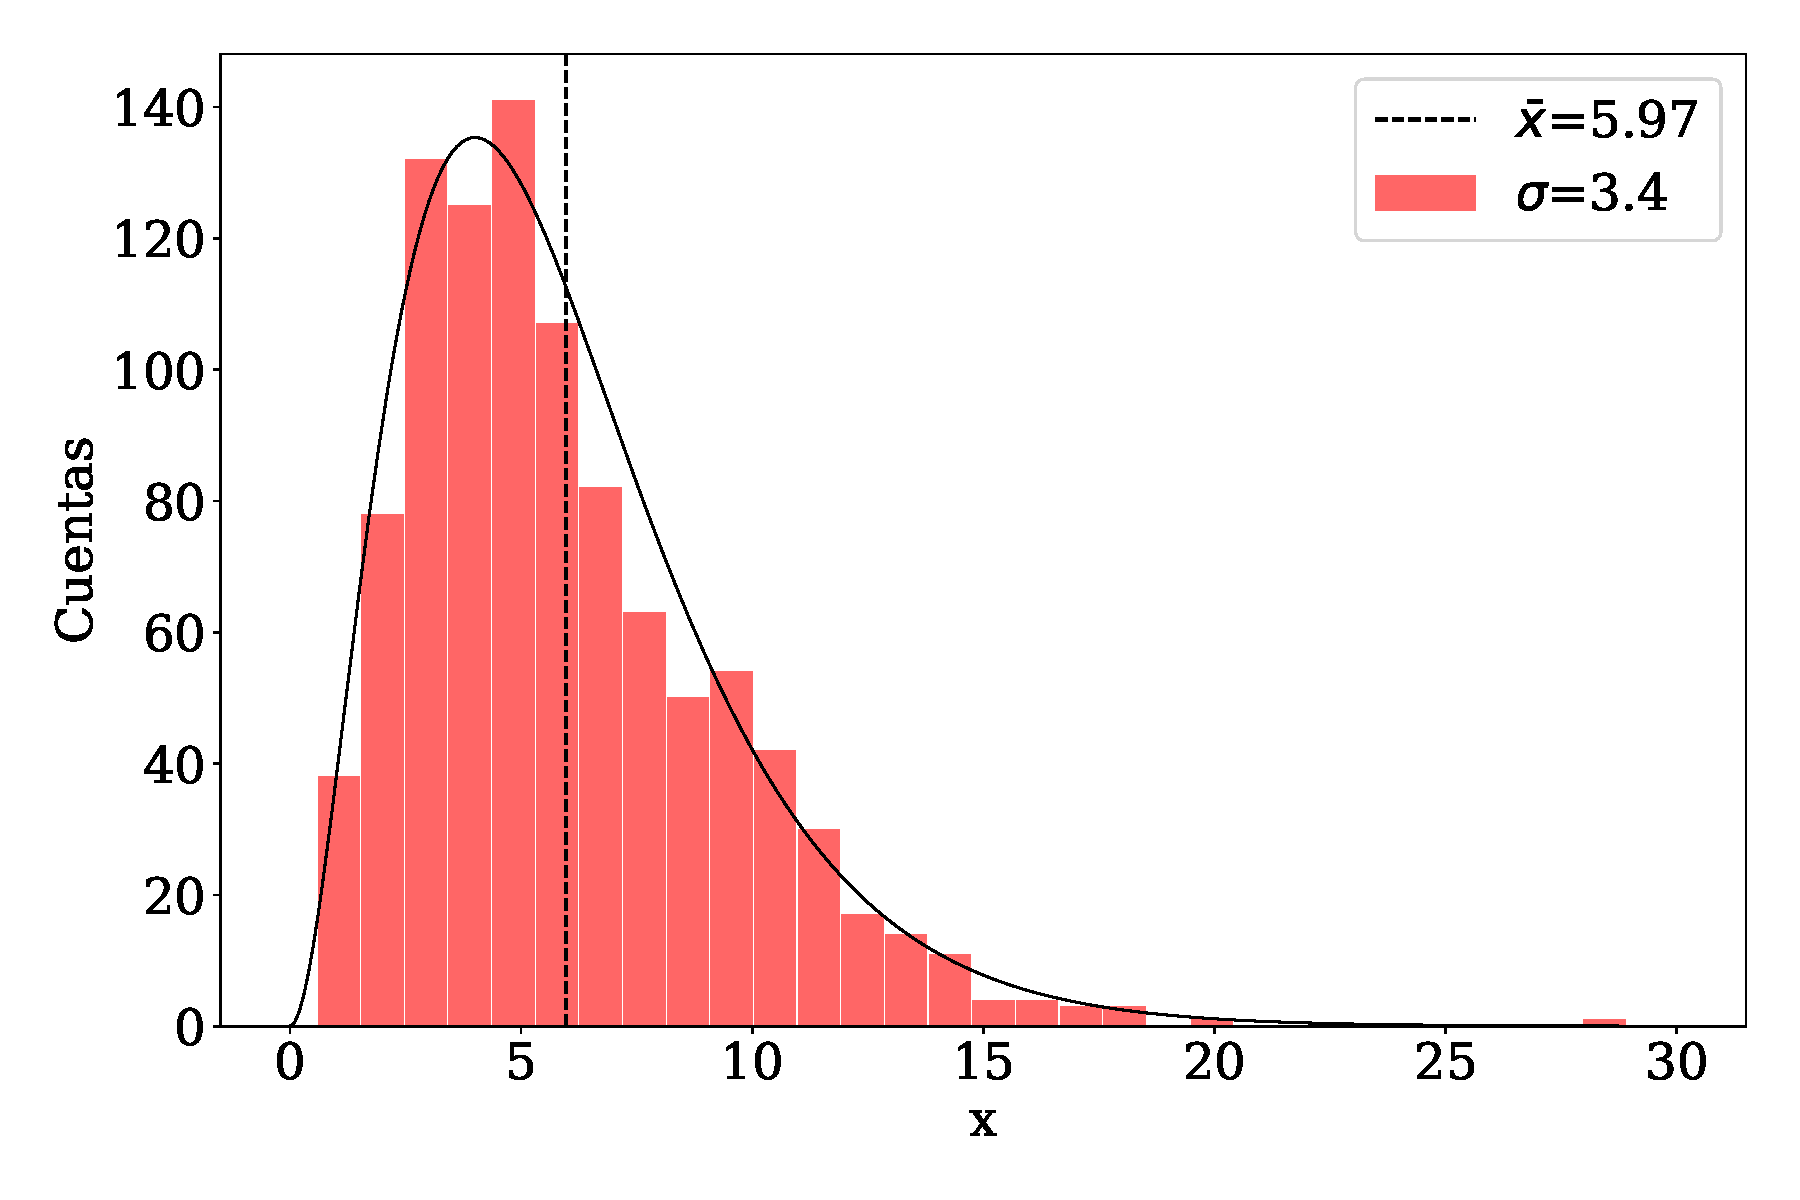
\includegraphics[width=0.4\textwidth]{ejer_2_2.pdf}
	\caption{Ejercicio 2}
	\label{fig:ejer2}
\end{figure}
	

\section*{Ejercicio 3 y 4}
 
El ejercicio 3 consiste en resolver un ecuación cuadrática $ax^2+bx+c=0$ dada la fórmula, donde los parámetros $b$ y $c$ son opcionales. El ejercicio 4 consiste en graficar la función y ubicar sus raíces en el mismo gráfico. 

Para realizar estos ejercicios, se implementaron las siguientes funciones para garantizar la validez de los parámetros ingresados por el usuario.
\begin{itemize}
	\item \verb|parametros()|:

		Esta función verifica que los parámetros $a$, $b$ y $c$ ingresados por el usuario sean válidos. Para  el caso de $b$ y $c$, al no ser inicializados, toman un valor predeterminado nulo.
	\item \verb|cuadratica(a,b,c)|:


		Verifica que la ecuación tenga al menos una solución real. Si existen devuelve un \verb|array|  con las soluciones, caso contrario devuelve \verb|None|
\end{itemize}


Una vez que el usuario ingresó los parámetros correctamente y se verificó que la ecuación tiene al menos una solución real, se puede graficar la cuadrática y sus raíces.
En la Fig.\ref{fig:ejer4} se muestra $f(x) = 3x^2+5x-1$ y sus raíces. Para graficar las mismas se utilizó la función \verb|scatter|, para las flechas \verb|annotate| y las anotaciones \verb|text|. No se utiliza \verb|annotate| para el texto porque la función \verb|text| deja un mejor aspecto en el caja que contiene al texto.

\begin{figure}[H]
	\centering
	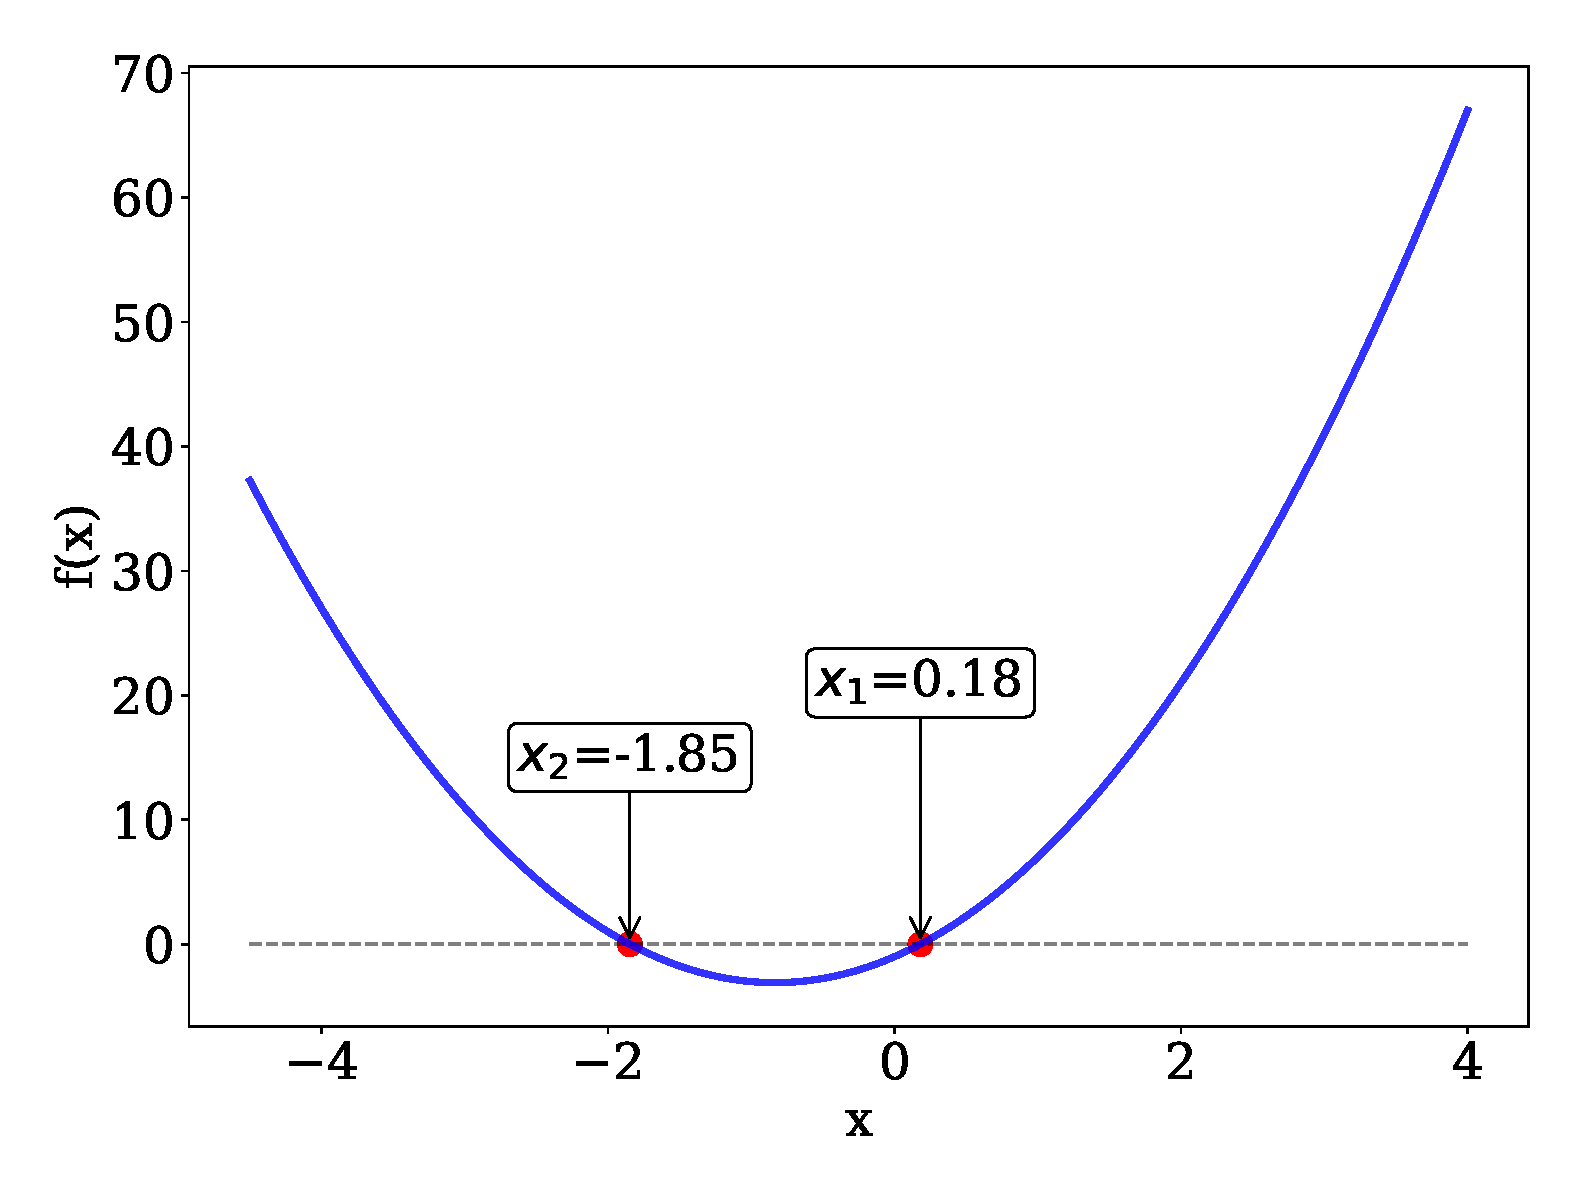
\includegraphics[width=0.4\textwidth]{ejer_4.pdf}
	\caption{Ejercicio 4}
	\label{fig:ejer4}
\end{figure}
	

\section*{Ejercicio 5}

En este ejercicio se inicializa la clase \verb|Lineal| que busca implementar una función lineal $f(x) = ax+b$. Dentro de esta clase se definen las siguientes funciones:
\begin{itemize}
	\item \verb|solucion(y)|:
		Dado los parámetros $a$ y $b$ y un valor de $f(x)=y$, se calcula el valor de $x$. Este programa tiene una ``flag'' cuando el parámetro $a=0$, donde la solución no está definida.

	\item \verb|f(x)|:		Evalúa la expresión dado un x.

	\item \_\_\verb|str|\_\_: 		Imprime la expresión $f(x) = ax+b$ a la salida.
\end{itemize}

\section*{Ejercicio 6}

Este ejercicio es análogo al anterior, salvo que la clase es \verb|Exponencial| y la expresión es $f(x)=ax^b$.


\section*{Ejercicio 7}

Para este ejercicio se creo un librería llamada \verb|circunferencia.py|, donde se definen la constante \verb|PI|, que equivale a $\pi$, y la función \verb|area(r)| que acepta el valor del radio y devuelve al área.

En la implementación se importan la constante y la función del área de dos formas distintas: 
\begin{itemize}
	\item \verb|import circunferencia as circle|
	\item \verb|from circunferencia import area, PI|
\end{itemize}
Se observa que al  ejecutar el comando \verb|circle.PI is PI| se obtiene \verb|True|, análogamente para \verb|circle.area is area|, lo que indicarían que las formas de llamar a estas entidades devuelven el mismo tipo de constante o función.


\section*{Ejercicio 8}

Se creó un archivo llamado \verb|geometria.py|, donde se llamaron los módulos \verb|circunferencia| y \verb|rectangulo|.


\section*{Ejercicio 9}

Para generar la carpeta con la librería \verb|p0_lib|, primeramente se creo una carpeta con ese nombre. Se agregó un archivo en blanco llamado \_\_\verb|init|\_\_\verb|.py| para que Python inicialice la carpeta como librería.

Luego en el código principal de la práctica 0 \verb|practica_0_DNN_main.py| se llamó a esta librería, como indica la práctica, de manera exitosa.

\section*{Ejercicio 10}

Para graficar la Fig.\ref{fig:ejer10} se ejecutó el comando \verb|meshgrid| con  los vectores \verb|x| e \verb|y| inicializados en el código de la práctica. 

Al comando \verb|imshow| se agregó el parámetro de color \verb|bone|, además de agregar la barra de colores y quitar los números de los ejes.

\begin{figure}[H]
	\centering
	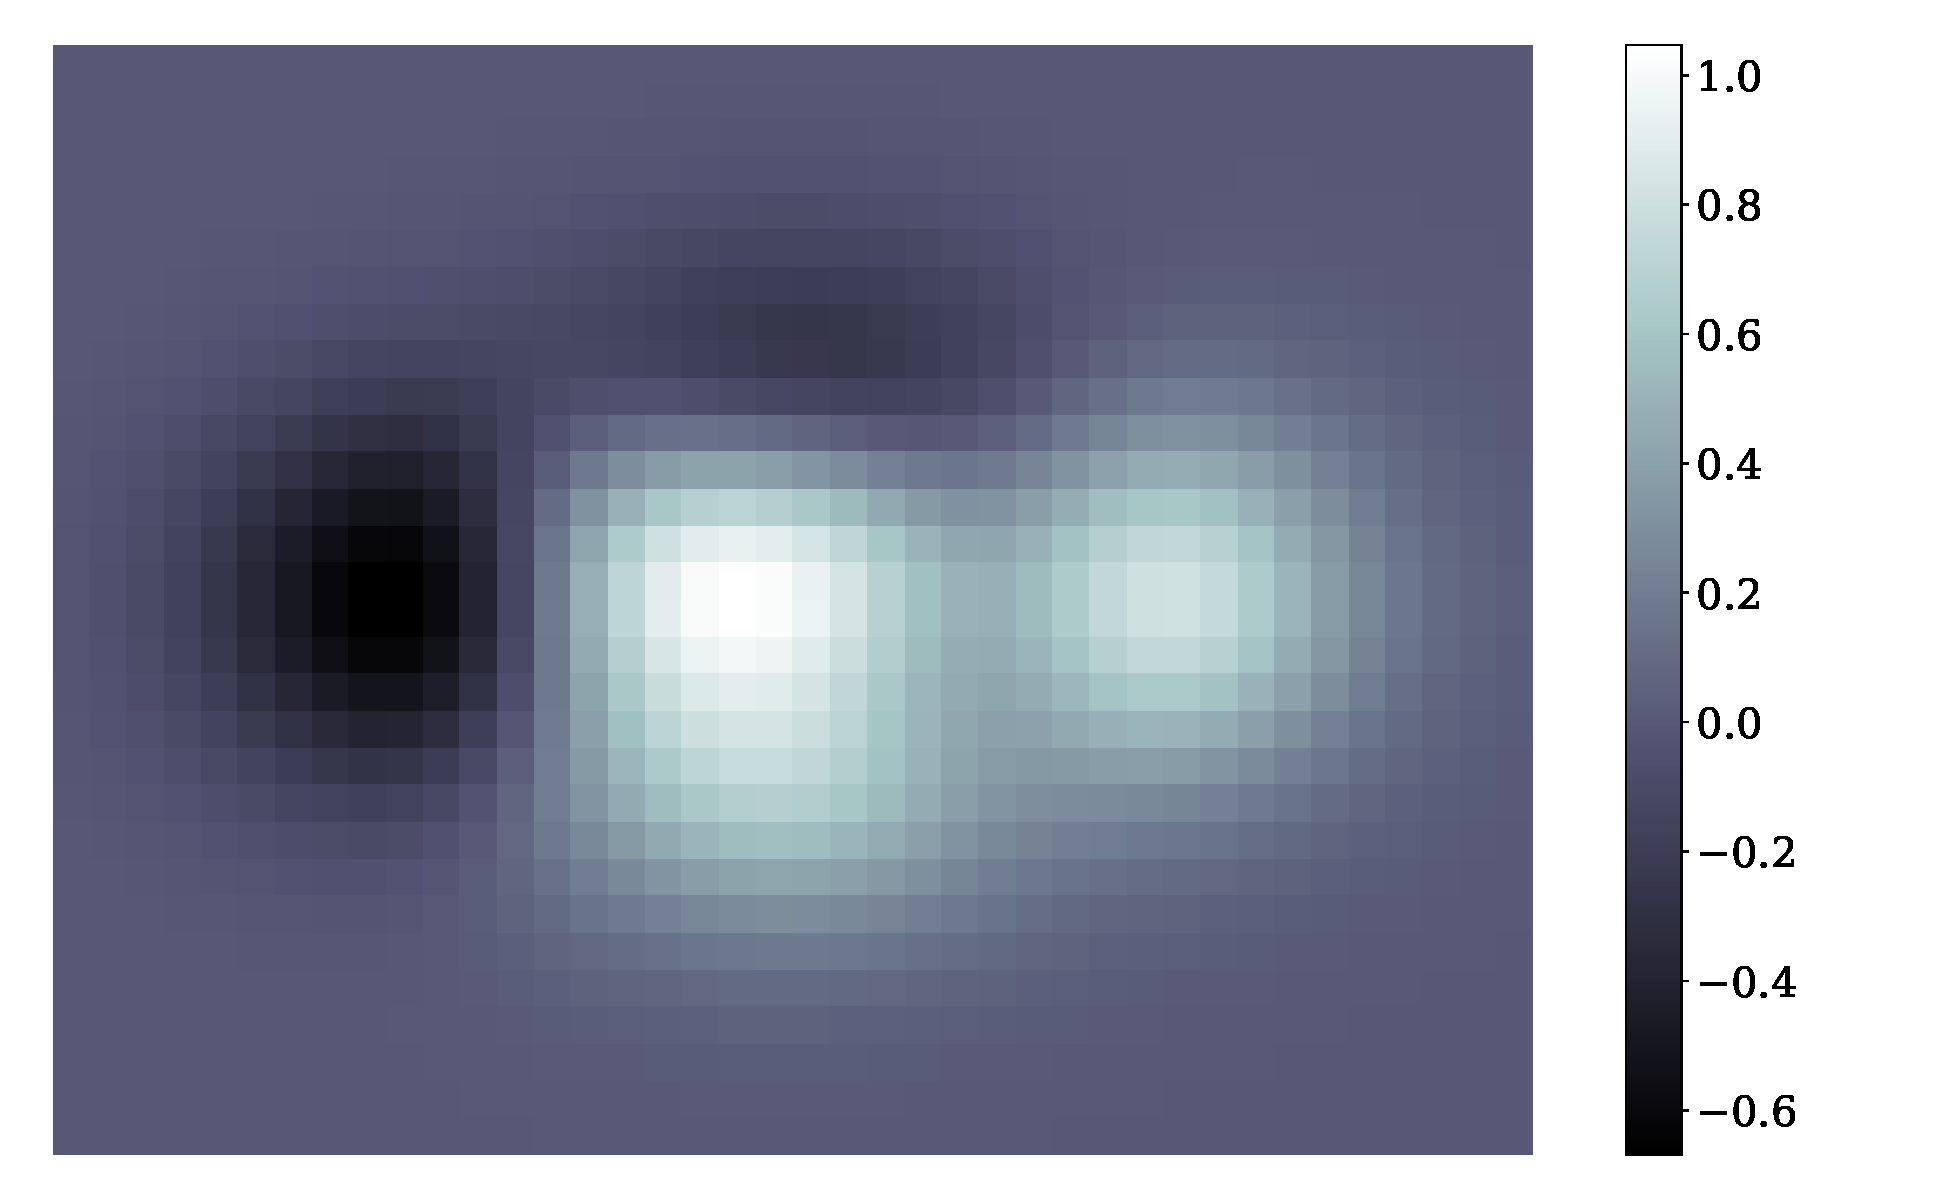
\includegraphics[width=0.5\textwidth]{ejer_10.pdf}
	\caption{Ejercicio 10}
	\label{fig:ejer10}
\end{figure}
	

\section*{Ejercicio 11}

Continuando con la función del ejercicio anterior, se usaron las funciones:

\begin{itemize}
	\item \verb|contourf|: para separar el gráfico en 6 zonas según el valor de la función.
	\item \verb|contour|: para dibujar las líneas y separar las zonas.
	\item \verb|clabel|: para agregar el valor que representan estas líneas en el gráfico.

\end{itemize}
De esta forma se obtuvo el gráfico presentado en la Fig.\,\ref{fig:ejer11}.

\begin{figure}[H]
	\centering
	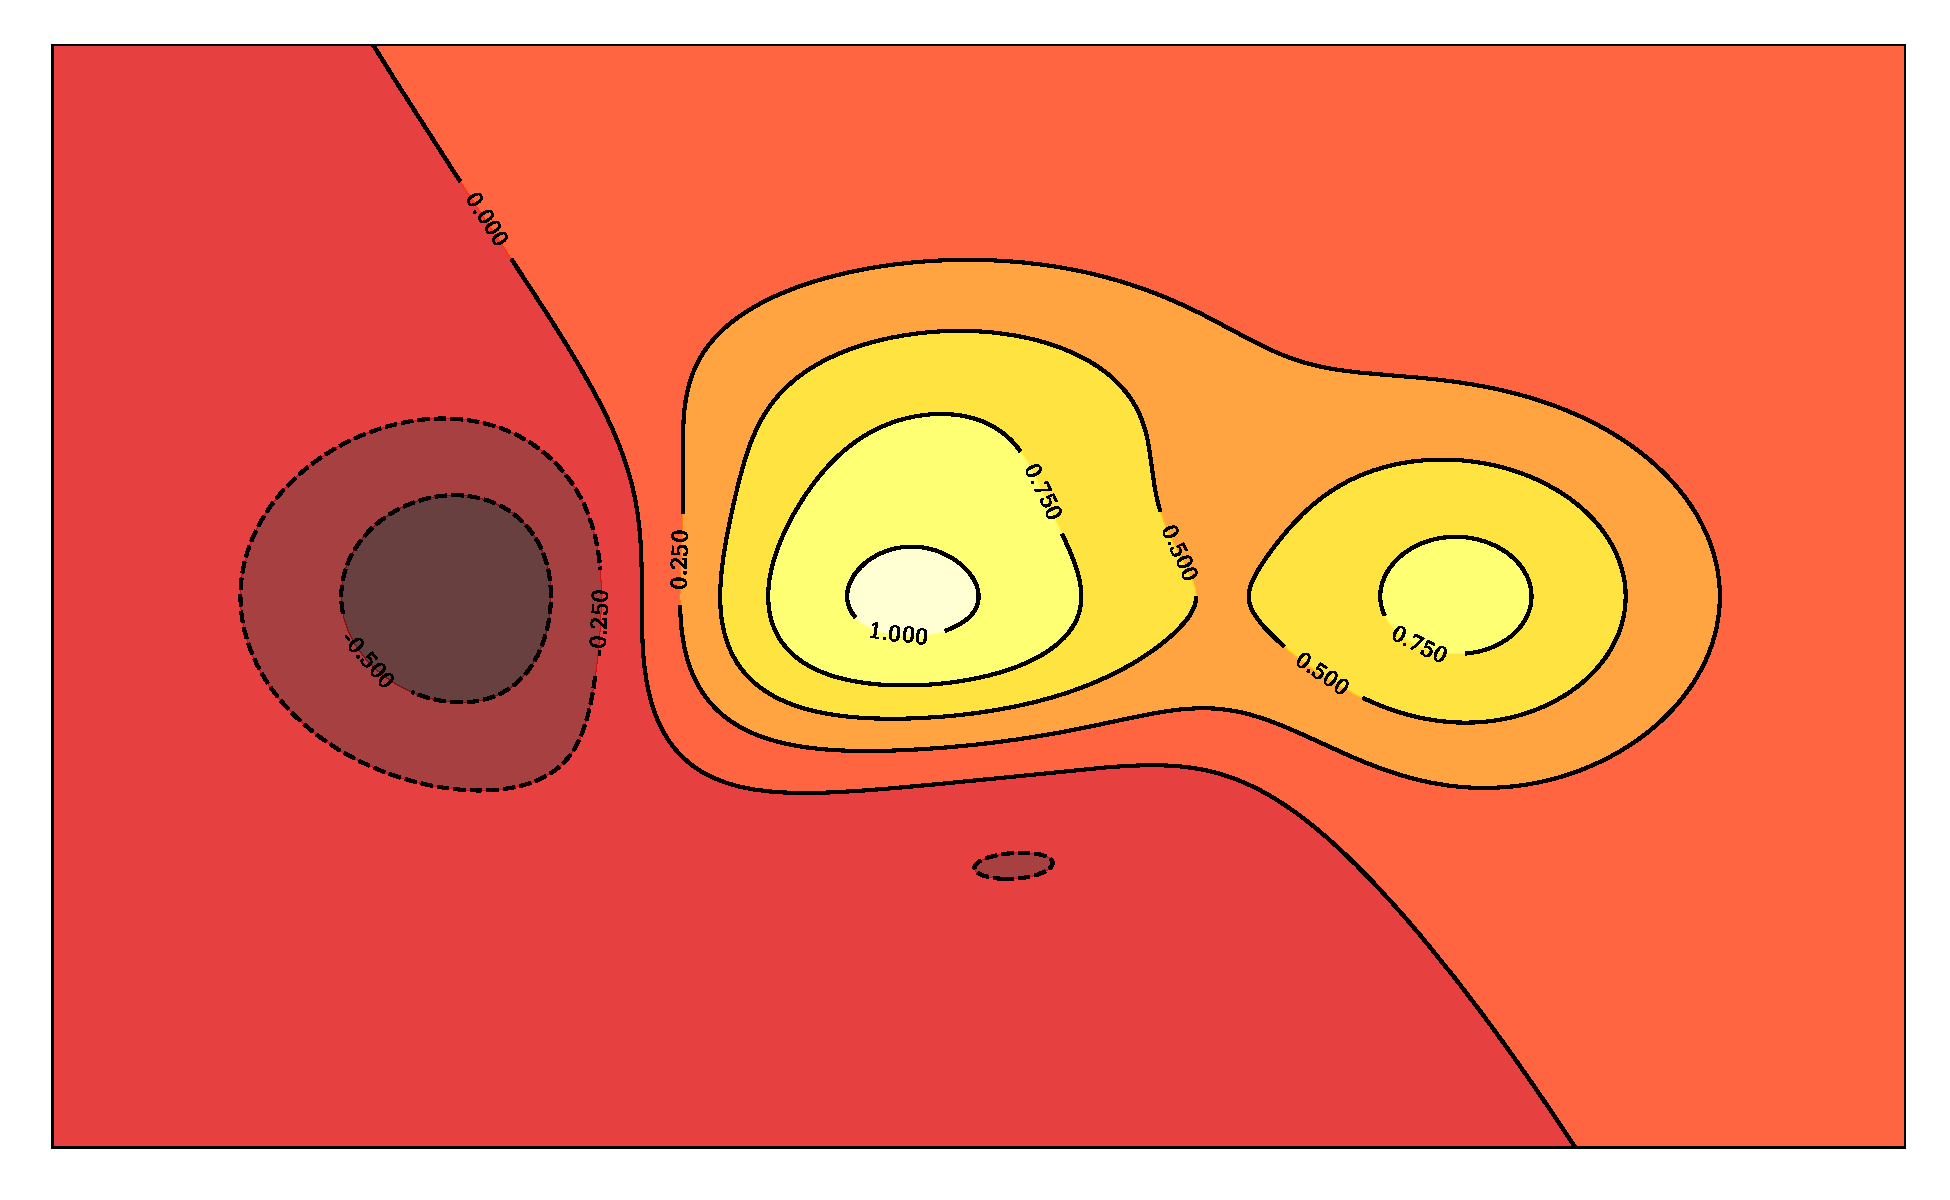
\includegraphics[width=0.5\textwidth]{ejer_11.pdf}
	\caption{Ejercicio 11}
	\label{fig:ejer11}
\end{figure}
	

\section*{Ejercicio 12}

Para realizar este gráfico, se tomaron 1024 puntos en el plano XY para graficarlos con la función \verb|scatter|. Usando el mapa de colores \verb|jet|, un tamaño de puntos $70$ y que cada punto se le asigne un color por su ángulo mediante la función \verb|arctan2(x,y)| se obtiene la Fig.\,\ref{fig:ejer12}.

\begin{figure}[H]
	\centering
	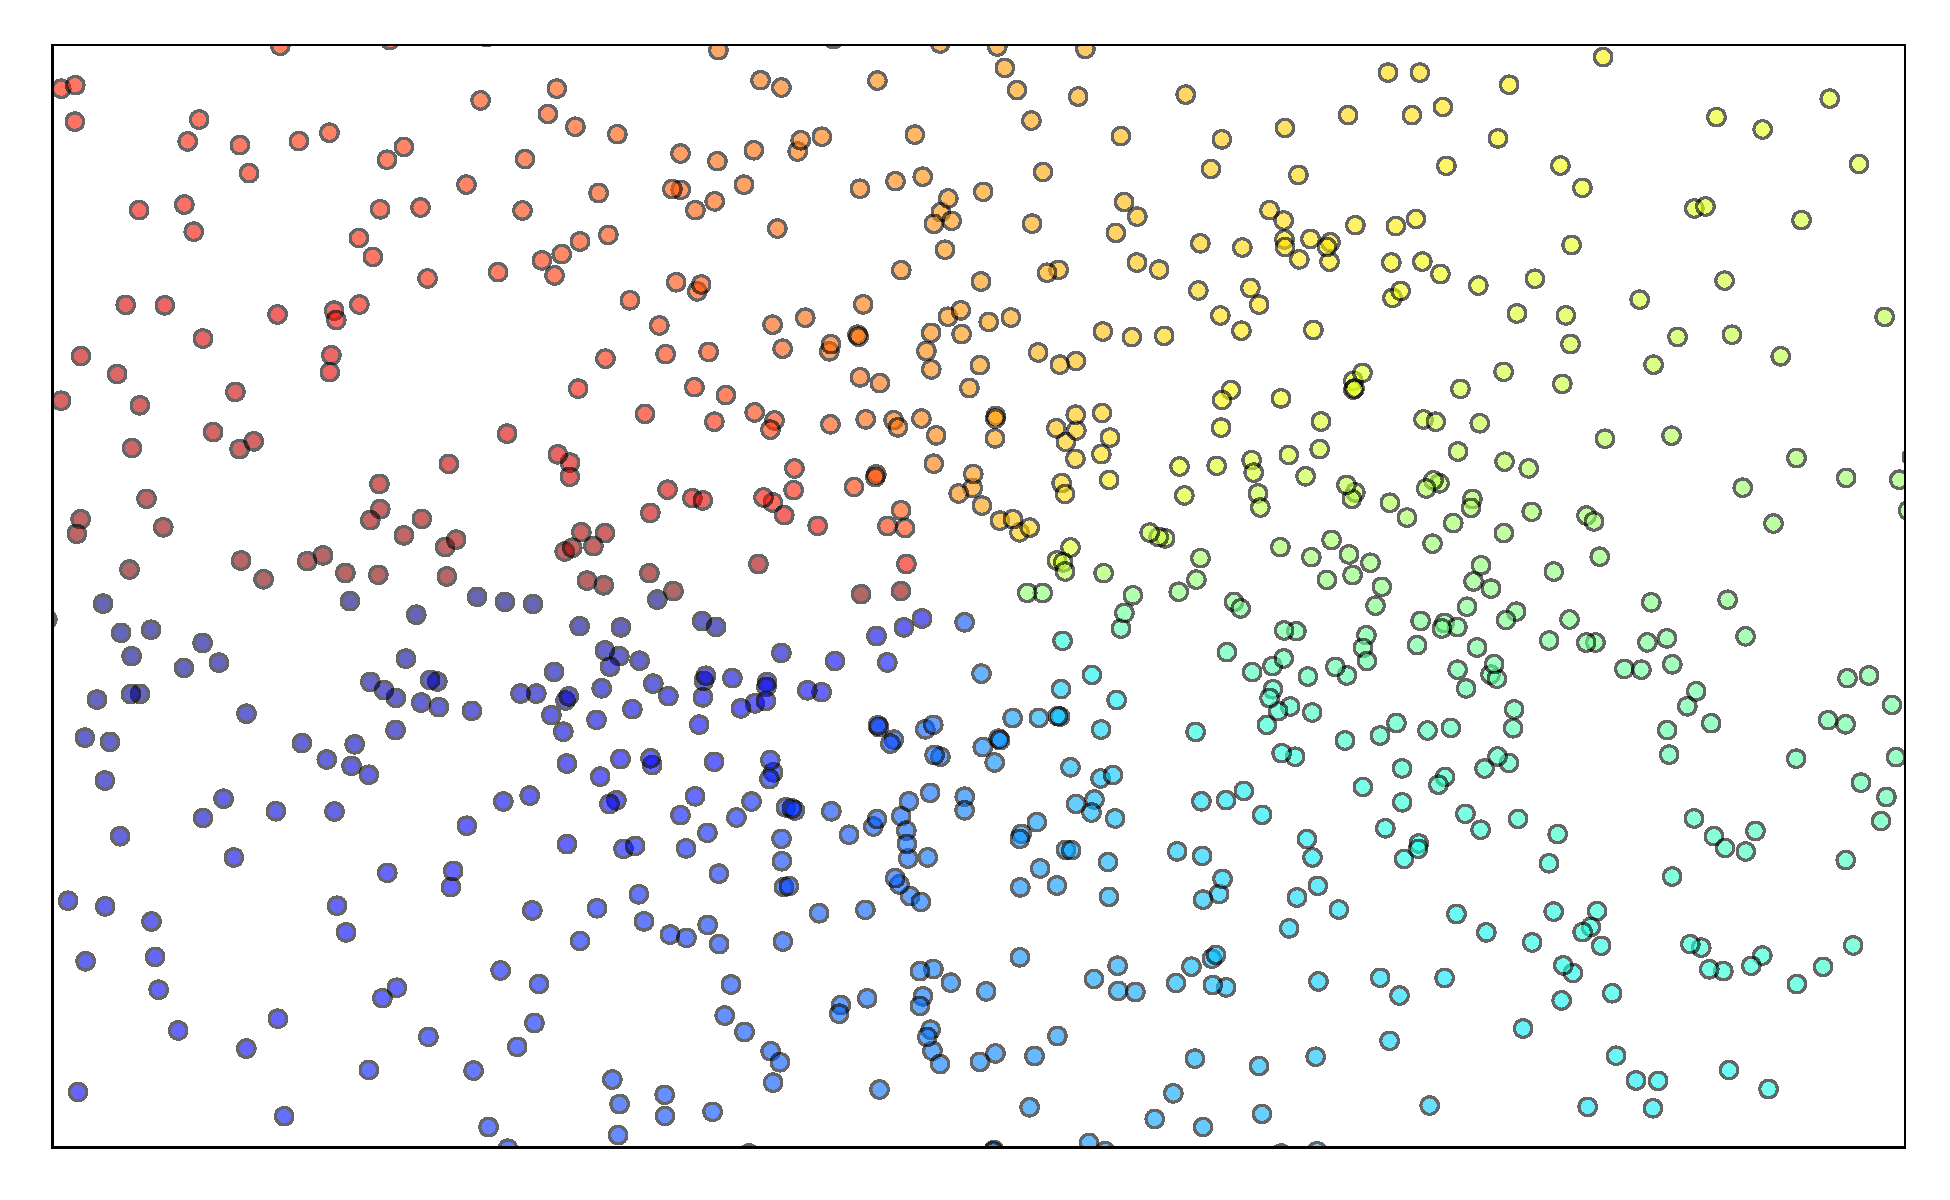
\includegraphics[width=0.5\textwidth]{ejer_12.pdf}
	\caption{Ejercicio 12}
	\label{fig:ejer12}
\end{figure}
	

\section*{Ejercicio 13}

En este ejercicio se simula un modelo de juguete para el movimiento de un cardumen. El mismo consiste en 3 reglas, mencionadas en la práctica,  que limitan la velocidad que debe tener cada pez.

Esta simulación se creo una clase \verb|R2| que intenta recrear las operaciones usuales en vectores de dos dimensiones. Para ello, se utilizo el \emph{overloading} de funciones del tipo suma, resta, multiplicación y división por escalares.

También se creó una clase \verb|Pez|, que guarda la posición y velocidad  de un pez. Finalmente se creó también la clase \verb|Cardumen|, que guarda información sobre todos los peces y a su vez contiene métodos para modificar al cardumen.

Para la inicialización de los peces, se tomaron posiciones aleatorias dentro de un cuadrado de $40\times40$ y las velocidades aleatorias con un módulo menor a una velocidad límite \verb|maxVel=4|. Durante la ejecución del programa, para la actualización de la velocidad de un pez según la regla 2, se tuvieron en cuenta los peces que están a una distancia de \verb|d=3|.


Durante la ejecución del programa, se actualiza una ventana de \verb|matplotlib| en cada iteración, además se toma un tiempo muerto de $80\,$ms entre iteración para dar la impresión de ver  una simulación en vivo. De esta forma se facilita ver  la evolución del cardumen pero no es útil para guardar la animación en un archivo o para terminar la ejecución del programa sin correr todas las iteraciones.

\subsection*{Condiciones de contorno}

El enunciado del ejercicio no habla de las condiciones de contorno, por lo que en este  trabajo se simularon con  dos condiciones: paredes duras o sin paredes. La primera simularía a  un cardumen en un estanque, con la condición de que si llega a la pared, el sentido de la velocidad cambia. En cambio sin paredes, esta condición no se aplica

\subsubsection*{Sin paredes duras}

En este caso el cardumen puede moverse en todo el espacio. Durante la ejecución del código, la figura  que se esta imprimiendo sigue a los peces en caso de salirse del área inicial, como se ve en la Fig.\,\ref{fig:ejer13_sin}

\begin{figure}[H]
	\centering
	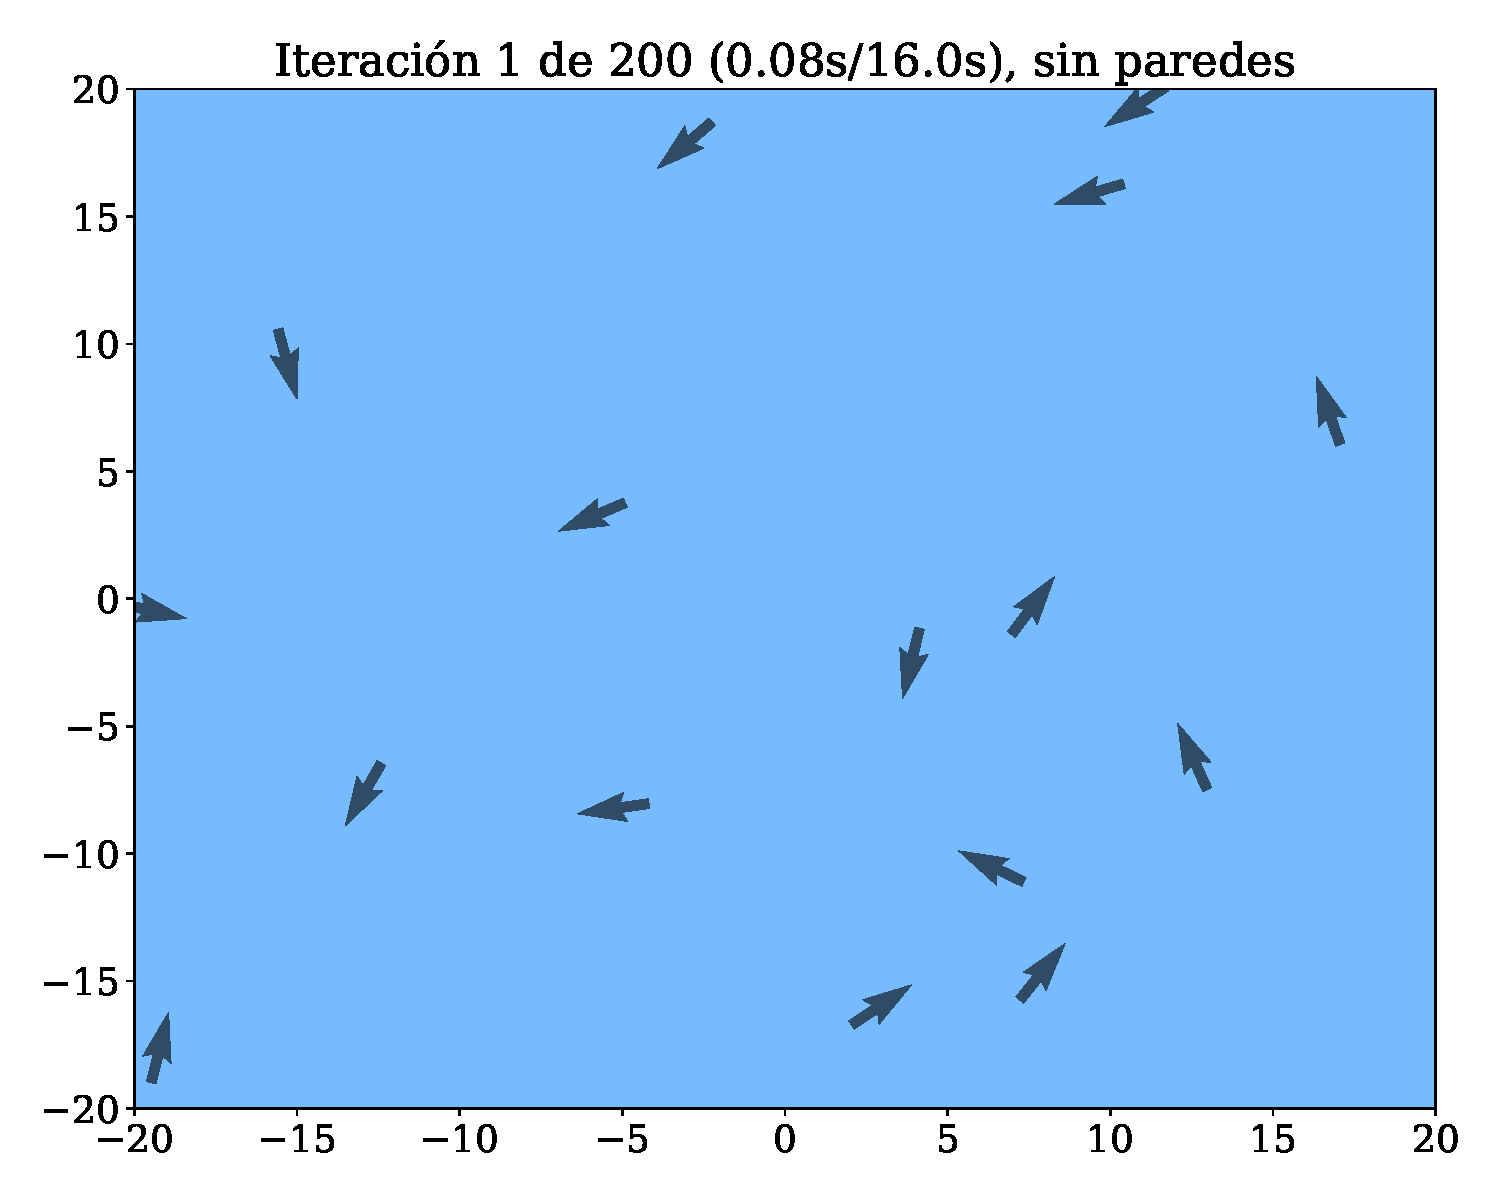
\includegraphics[width=0.41\textwidth]{ejer_13_0False.pdf}
	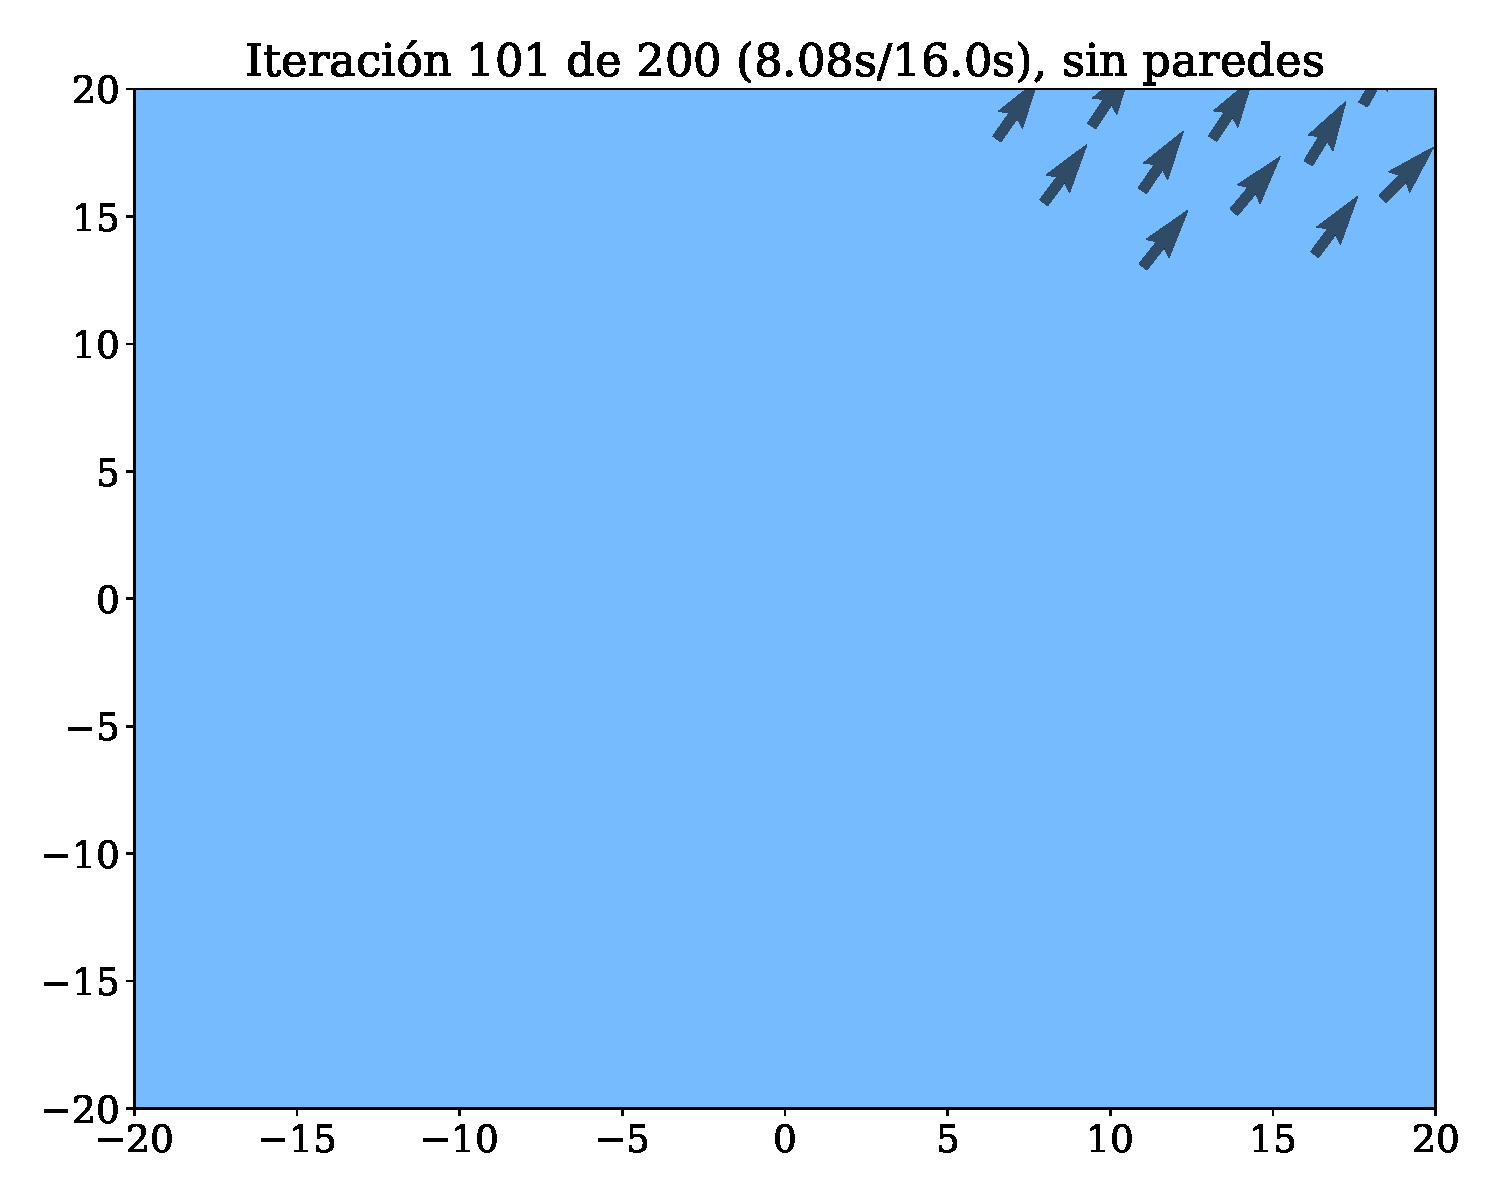
\includegraphics[width=0.41\textwidth]{ejer_13_100False.pdf}
	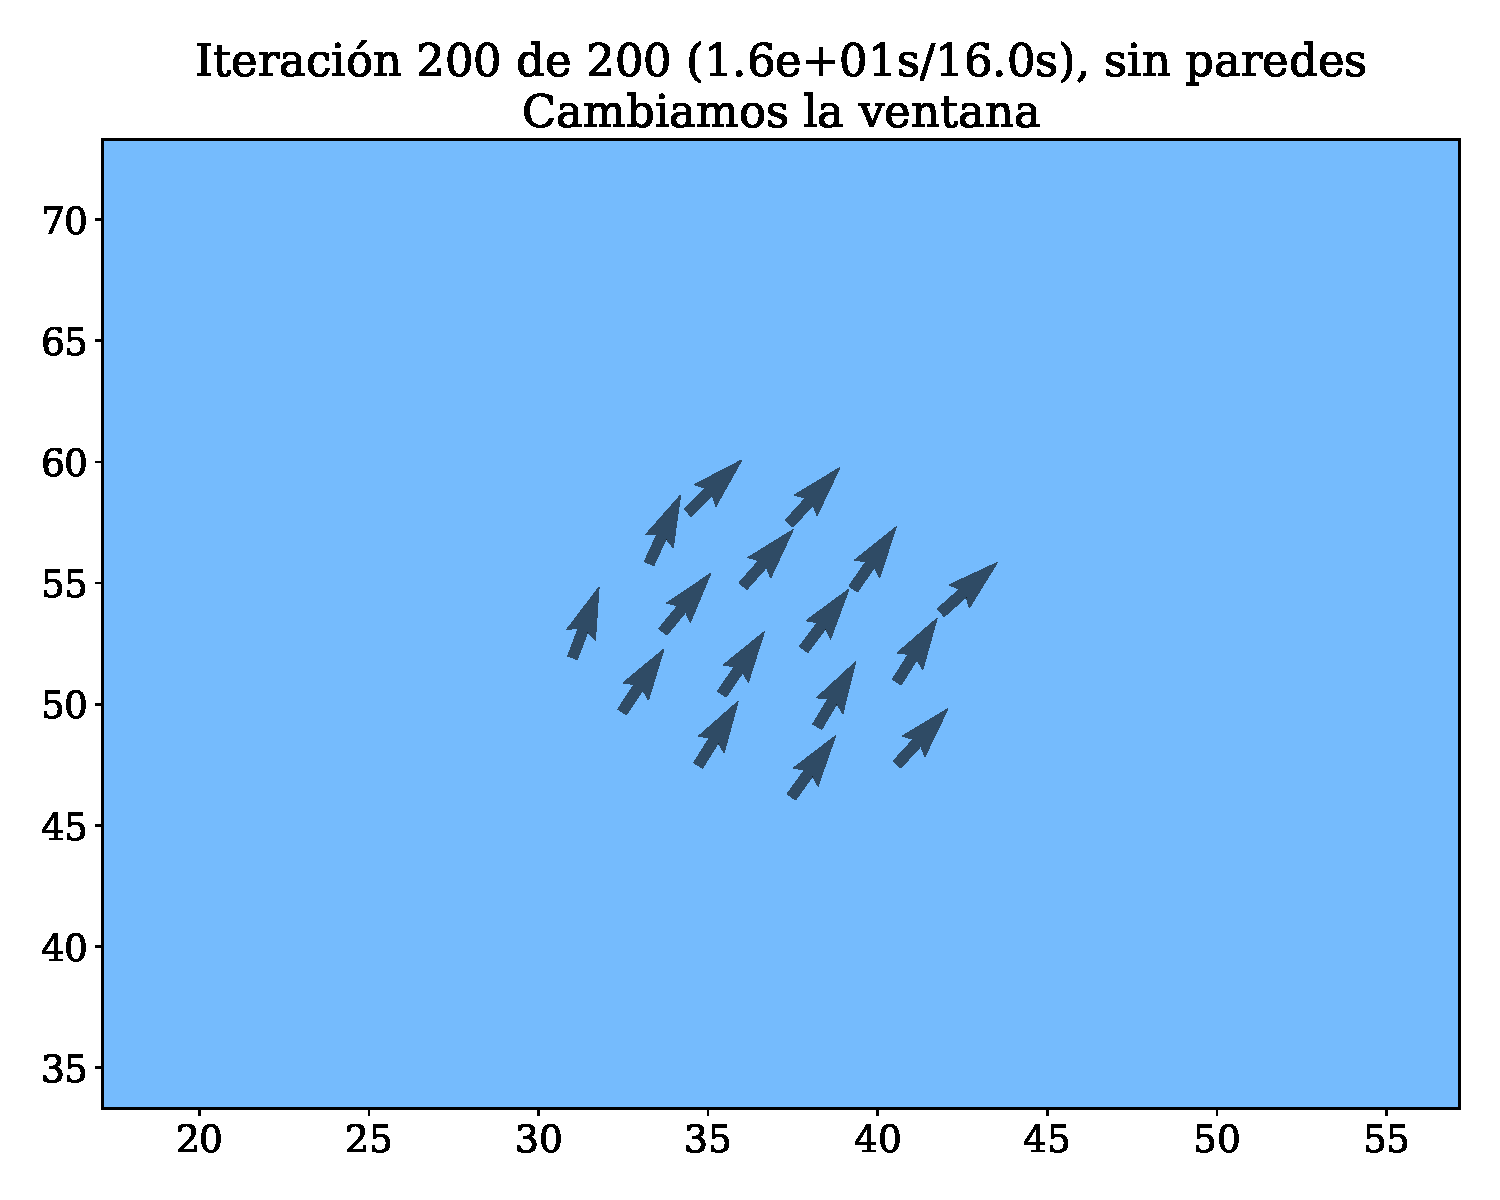
\includegraphics[width=0.41\textwidth]{ejer_13_199False.pdf}
	\caption{La simulación del ejercicio 13 sin considerar condiciones de contorno.}
	\label{fig:ejer13_sin}
\end{figure}

\subsubsection*{Con paredes duras}

Para este caso el comportamiento de los peces se ven afectado cuando llegan a la pared. En la Fig.\,\ref{fig:ejer13_con} se muestra que durante la mitad de la simulación, los peces se acercan con la pared, y ya para el final de la simulación se alejan de la pared que encontraron.

\begin{figure}[H]
	\centering
	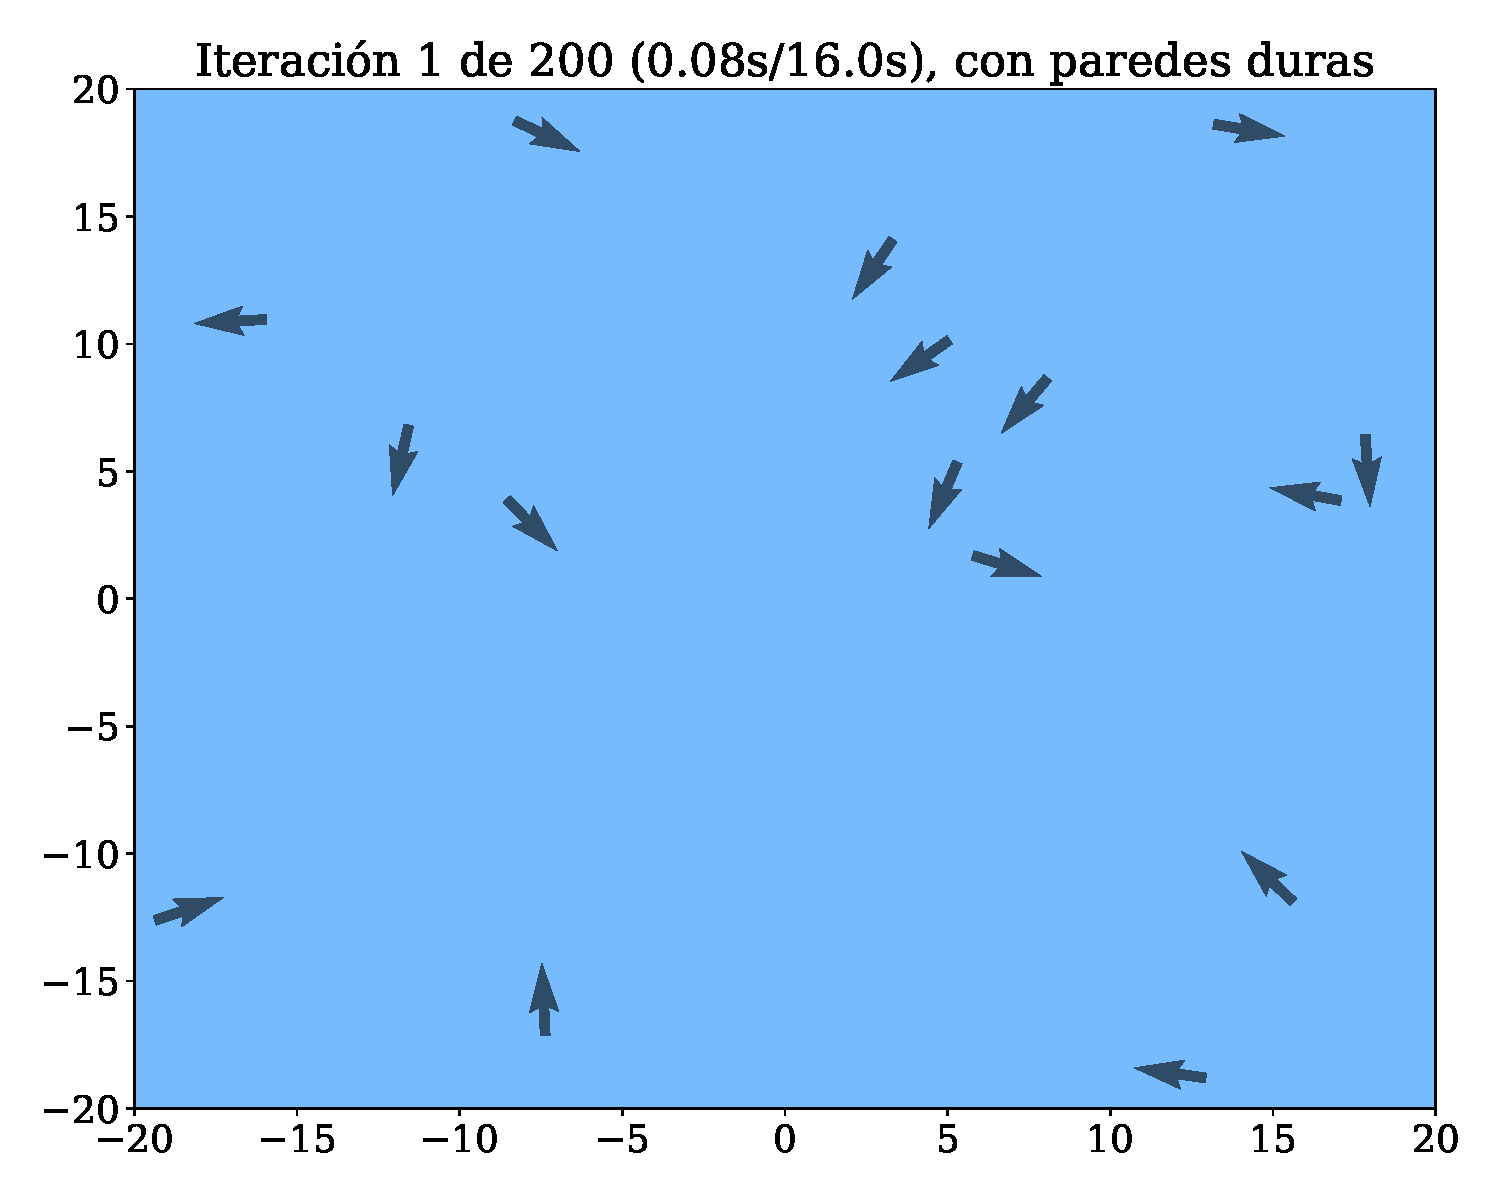
\includegraphics[width=0.41\textwidth]{ejer_13_0True.pdf}
	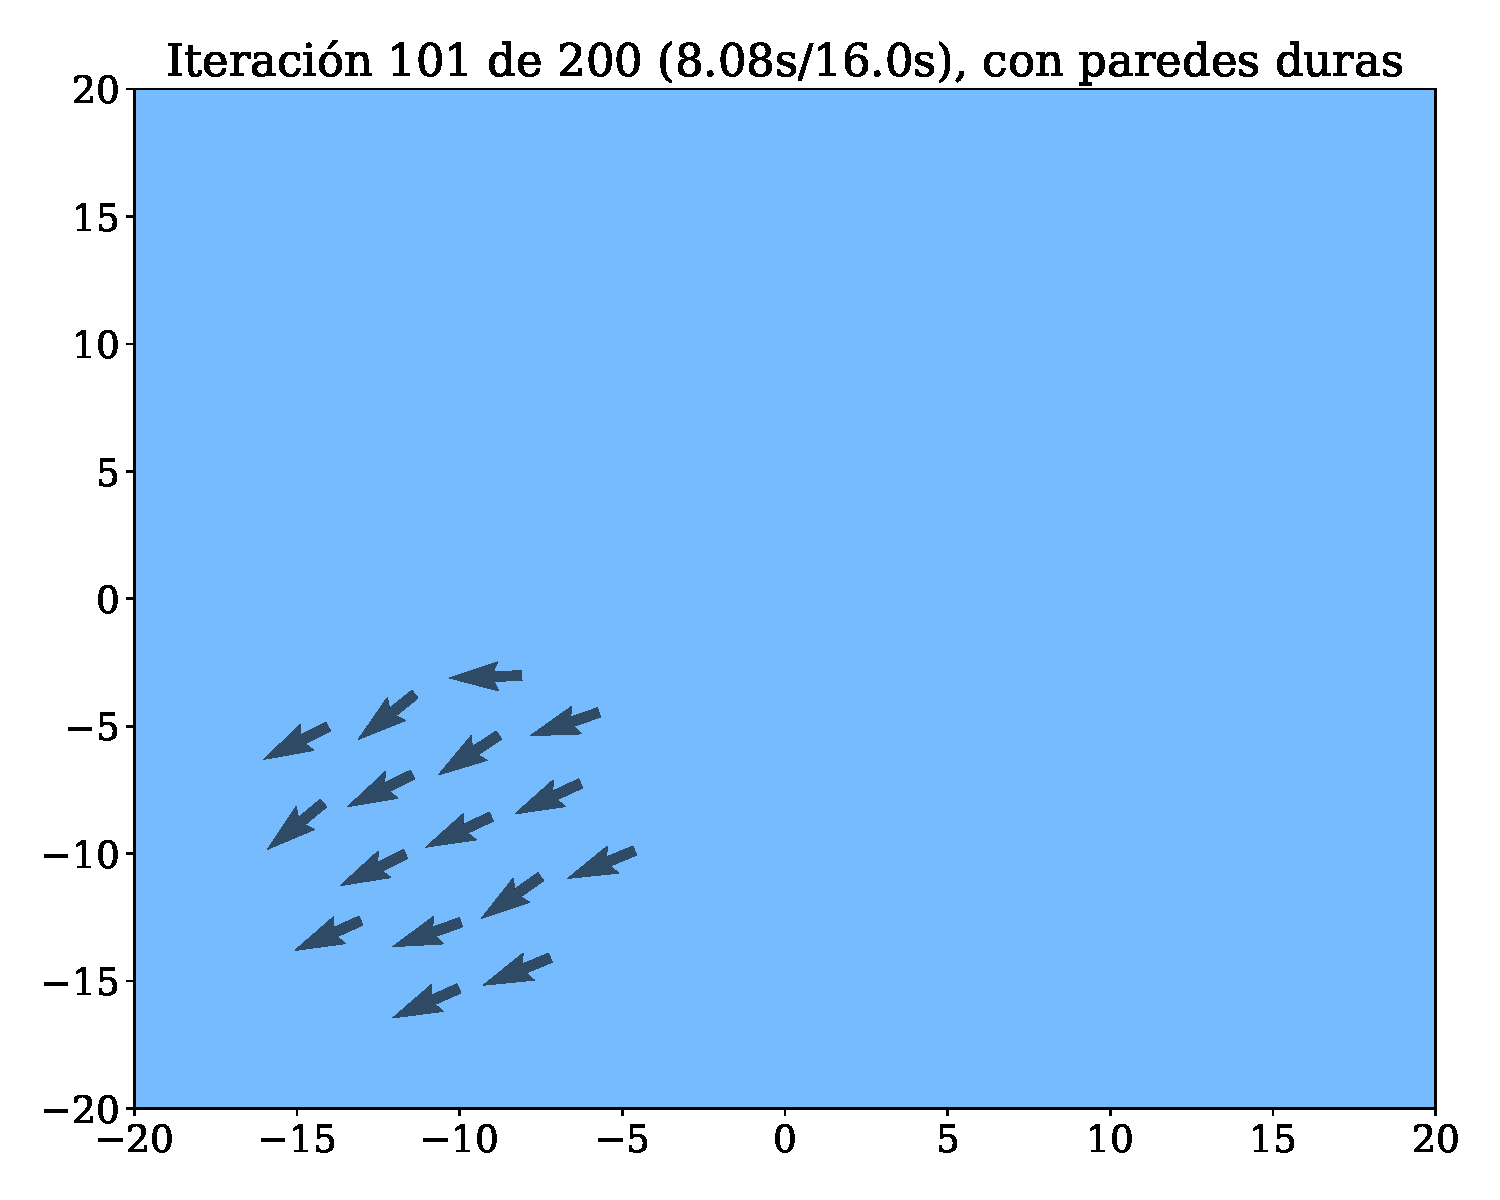
\includegraphics[width=0.41\textwidth]{ejer_13_100True.pdf}
	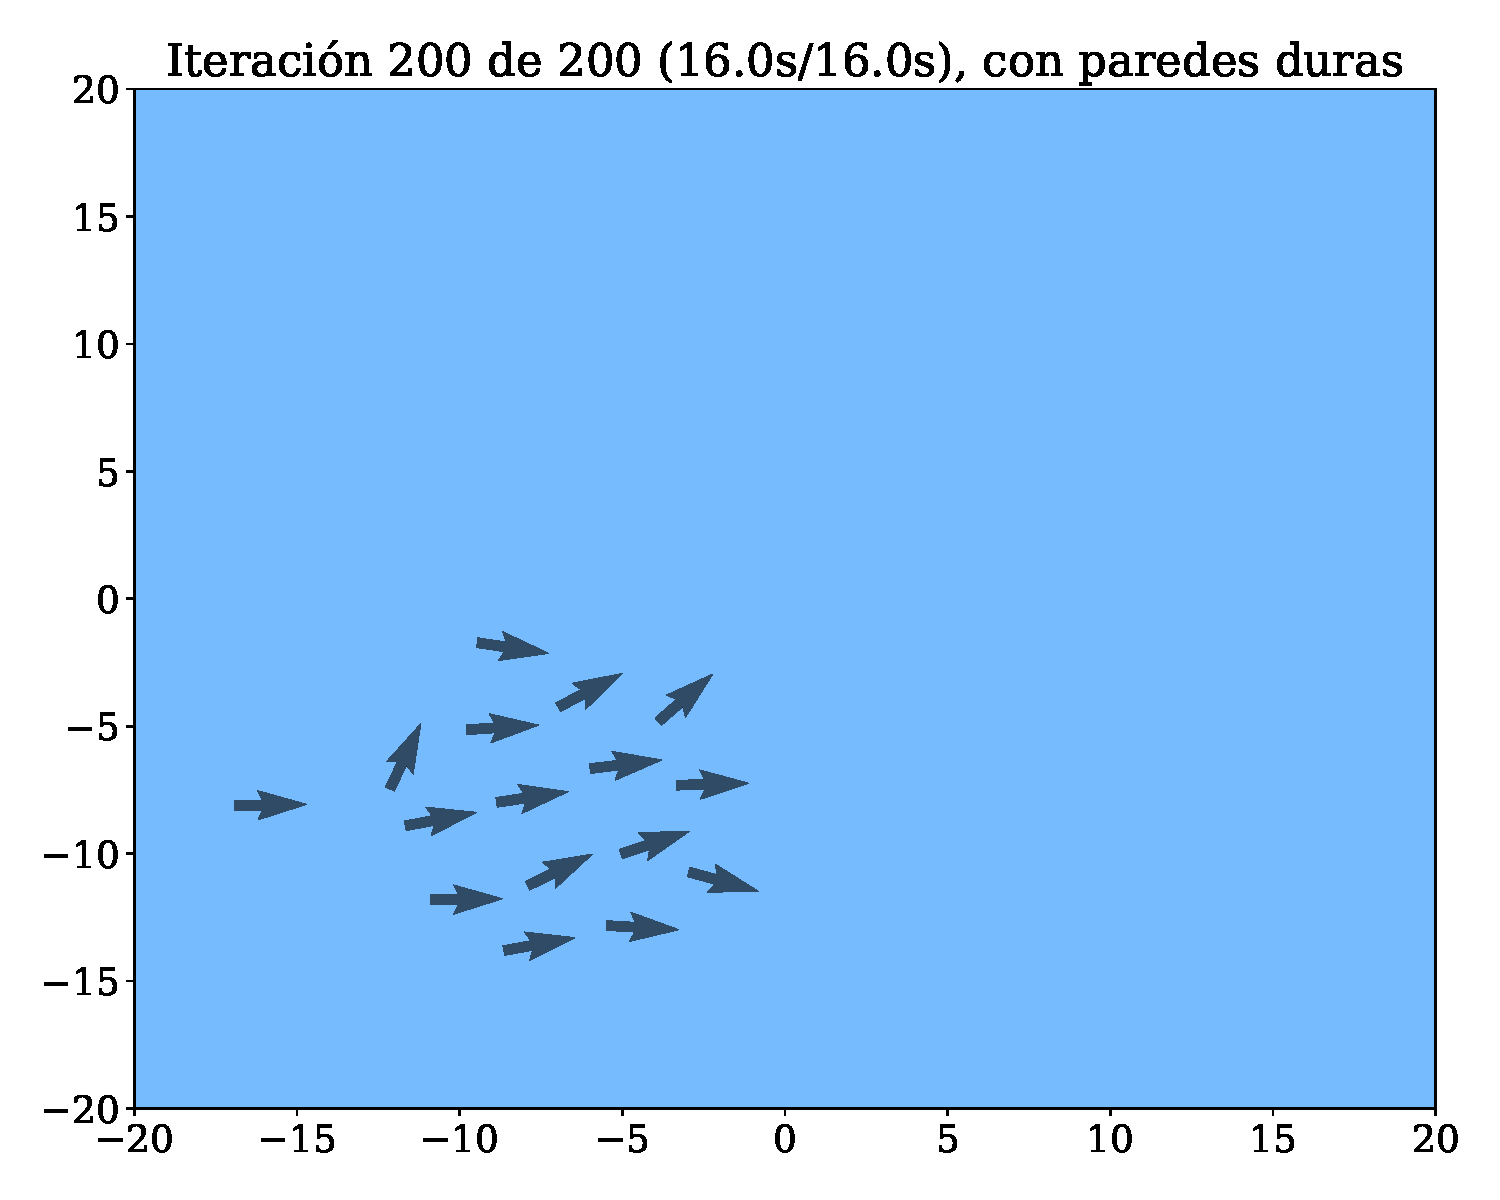
\includegraphics[width=0.41\textwidth]{ejer_13_199True.pdf}
	\caption{La simulación del ejercicio 13 considerando paredes duras como condiciones de contorno.}
	\label{fig:ejer13_con}
\end{figure}

\section*{Ejercicio 14}

Utilizando  la librería  \verb|numpy.random| se generaron números entre el 1 y 365, excluyendo así al posible caso donde alguien haya nacido el $29$ de Febrero, para ser asignados a las personas dentro de los grupos.

Una vez que cada persona se le asigna un día, se recorre grupo por grupo para verificar si existen por lo menos dos personas con el mismo número asignado, es decir, con el mismo cumpleaños.

La simulación arrojó las valores presentados en la Tabla\,\ref{tabla}. Como se observa en los datos, así como también en la Fig.\,\ref{fig:ejer14}, la probabilidad va convergiendo al $100\%$ a medida que se aumenta la cantidad de personas por grupo.

\begin{table}[h]
	\begin{tabular}{c|c}
Personas & Probabilidad \\ \hline
$10$ & $ 9.8\%$ \\ \hline
$20$ & $ 39.3\%$ \\ \hline
$30$ & $ 71.5\%$ \\ \hline
$40$ & $ 88.9\%$ \\ \hline
$50$ & $ 97.6\%$ \\ \hline
$60$ & $ 99.1\%$ \\ 
	\end{tabular}
\caption{Tabla de la cantidad de personas por grupo y la probabilidad que en ese grupo, dos personas hayan nacido el mismo día.}
\label{tabla}
\end{table}

\begin{figure}[H]
	\centering
	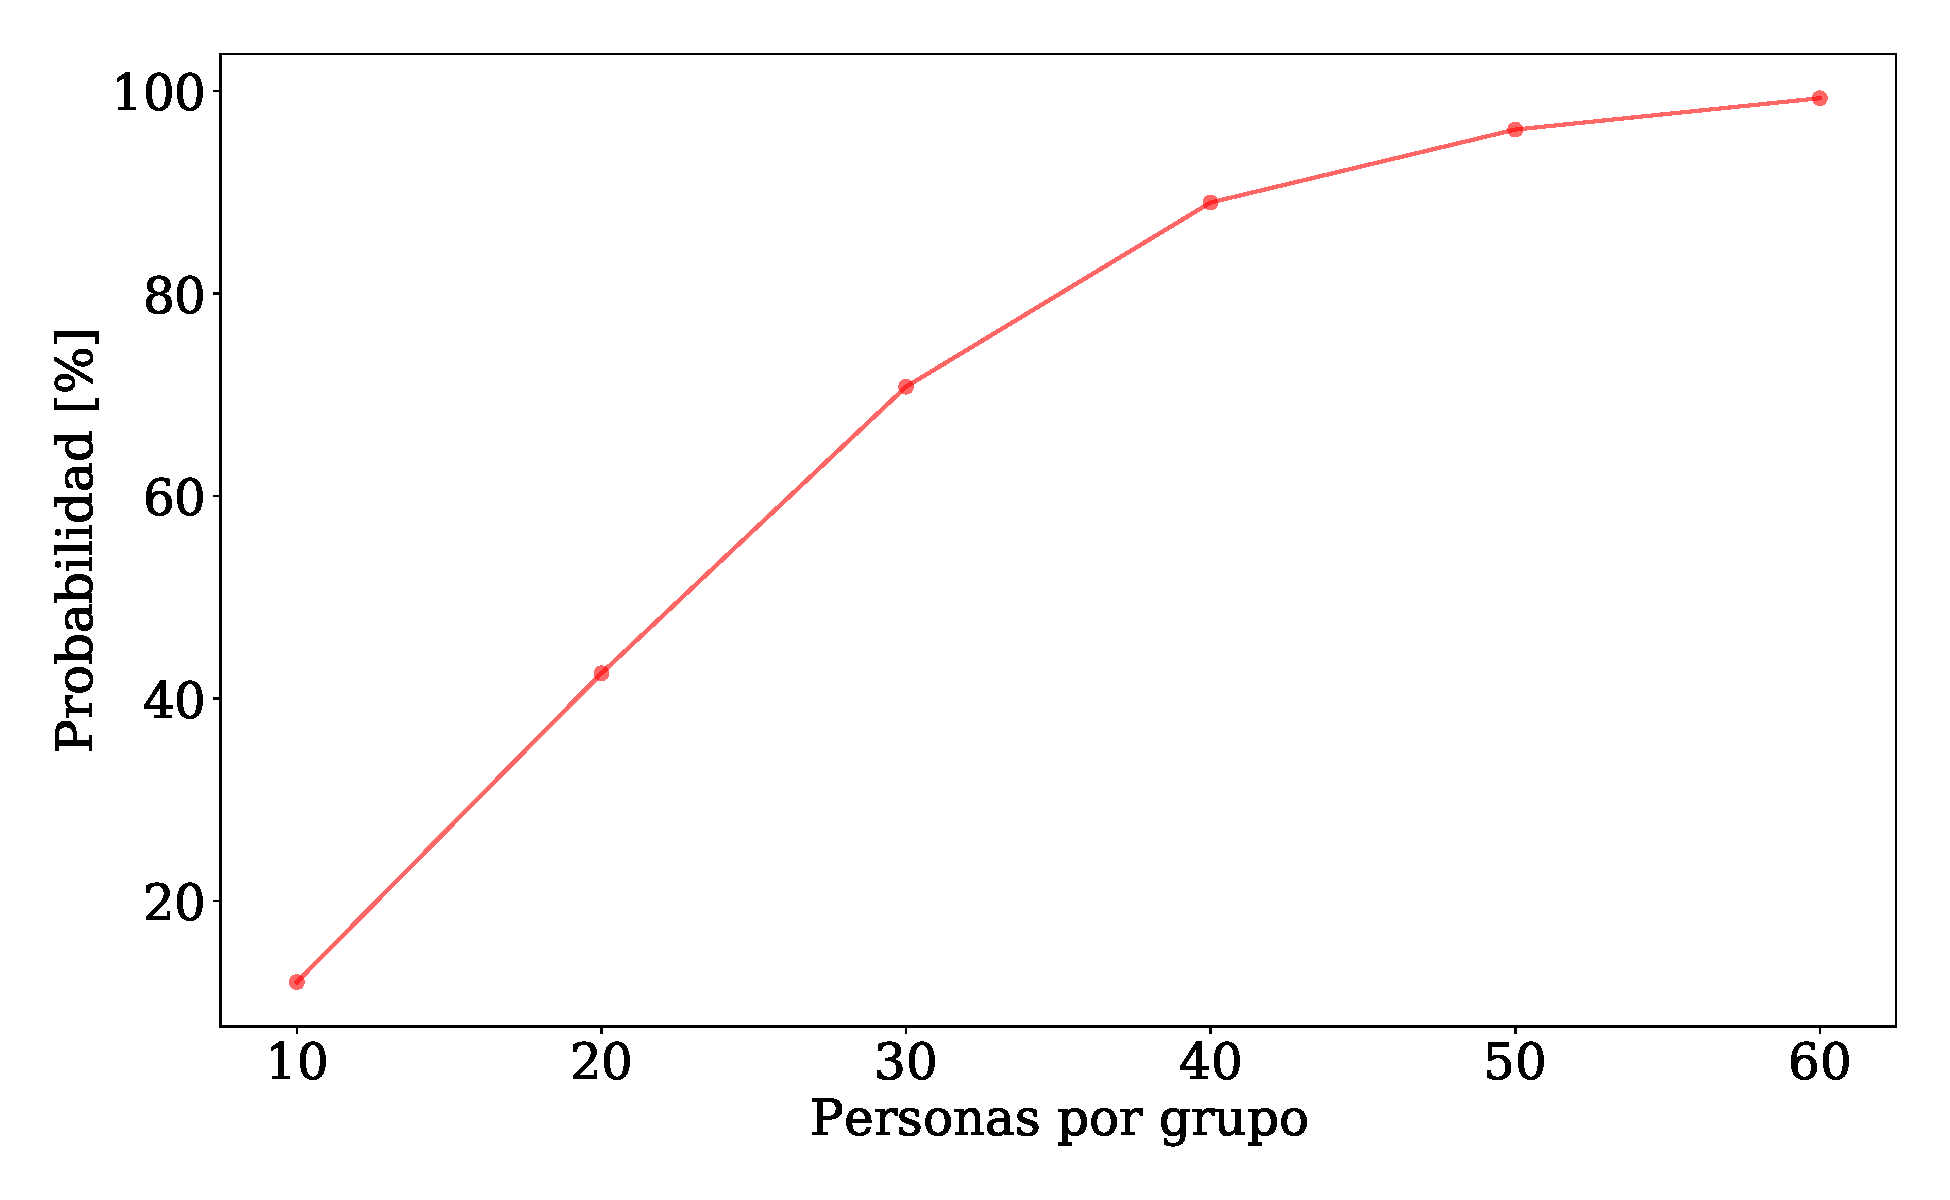
\includegraphics[width=0.45\textwidth]{ejer_14.pdf}
	\caption{Ejercicio 14}
	\label{fig:ejer14}
\end{figure}
	

\section*{Ejercicio 15}

Para este ejercicio se crearon dos clases, \verb|functor| y \verb|Noiser|, donde el último hereda las propiedades del primero. En la inicialización de \verb|functor| definimos los atributos \verb|minV| y \verb|maxV|, que en la función \_\_\verb|call|\_\_ se utilizan para devolver un número aleatorio entre estos dos valores.

Para la clase \verb|Noiser| se hereda la inicialización y para la función \_\_\verb|call|\_\_ acepta un argumento. Para la salida ahora se agrega la función \_\_\verb|call|\_\_ de functor y se suma el argumento.


Para poder usar estas clases y sus métodos sobre alguna señal almacenada en un \verb|array|, se utiliza la función \verb|np.vectorize|. En la Fig.\ref{fig:ejer15} se muestra una señal sinusoidal que pasó por el Noiser, con un ruido entre $[-0.2, 0.2]$

\begin{figure}[H]
	\centering
	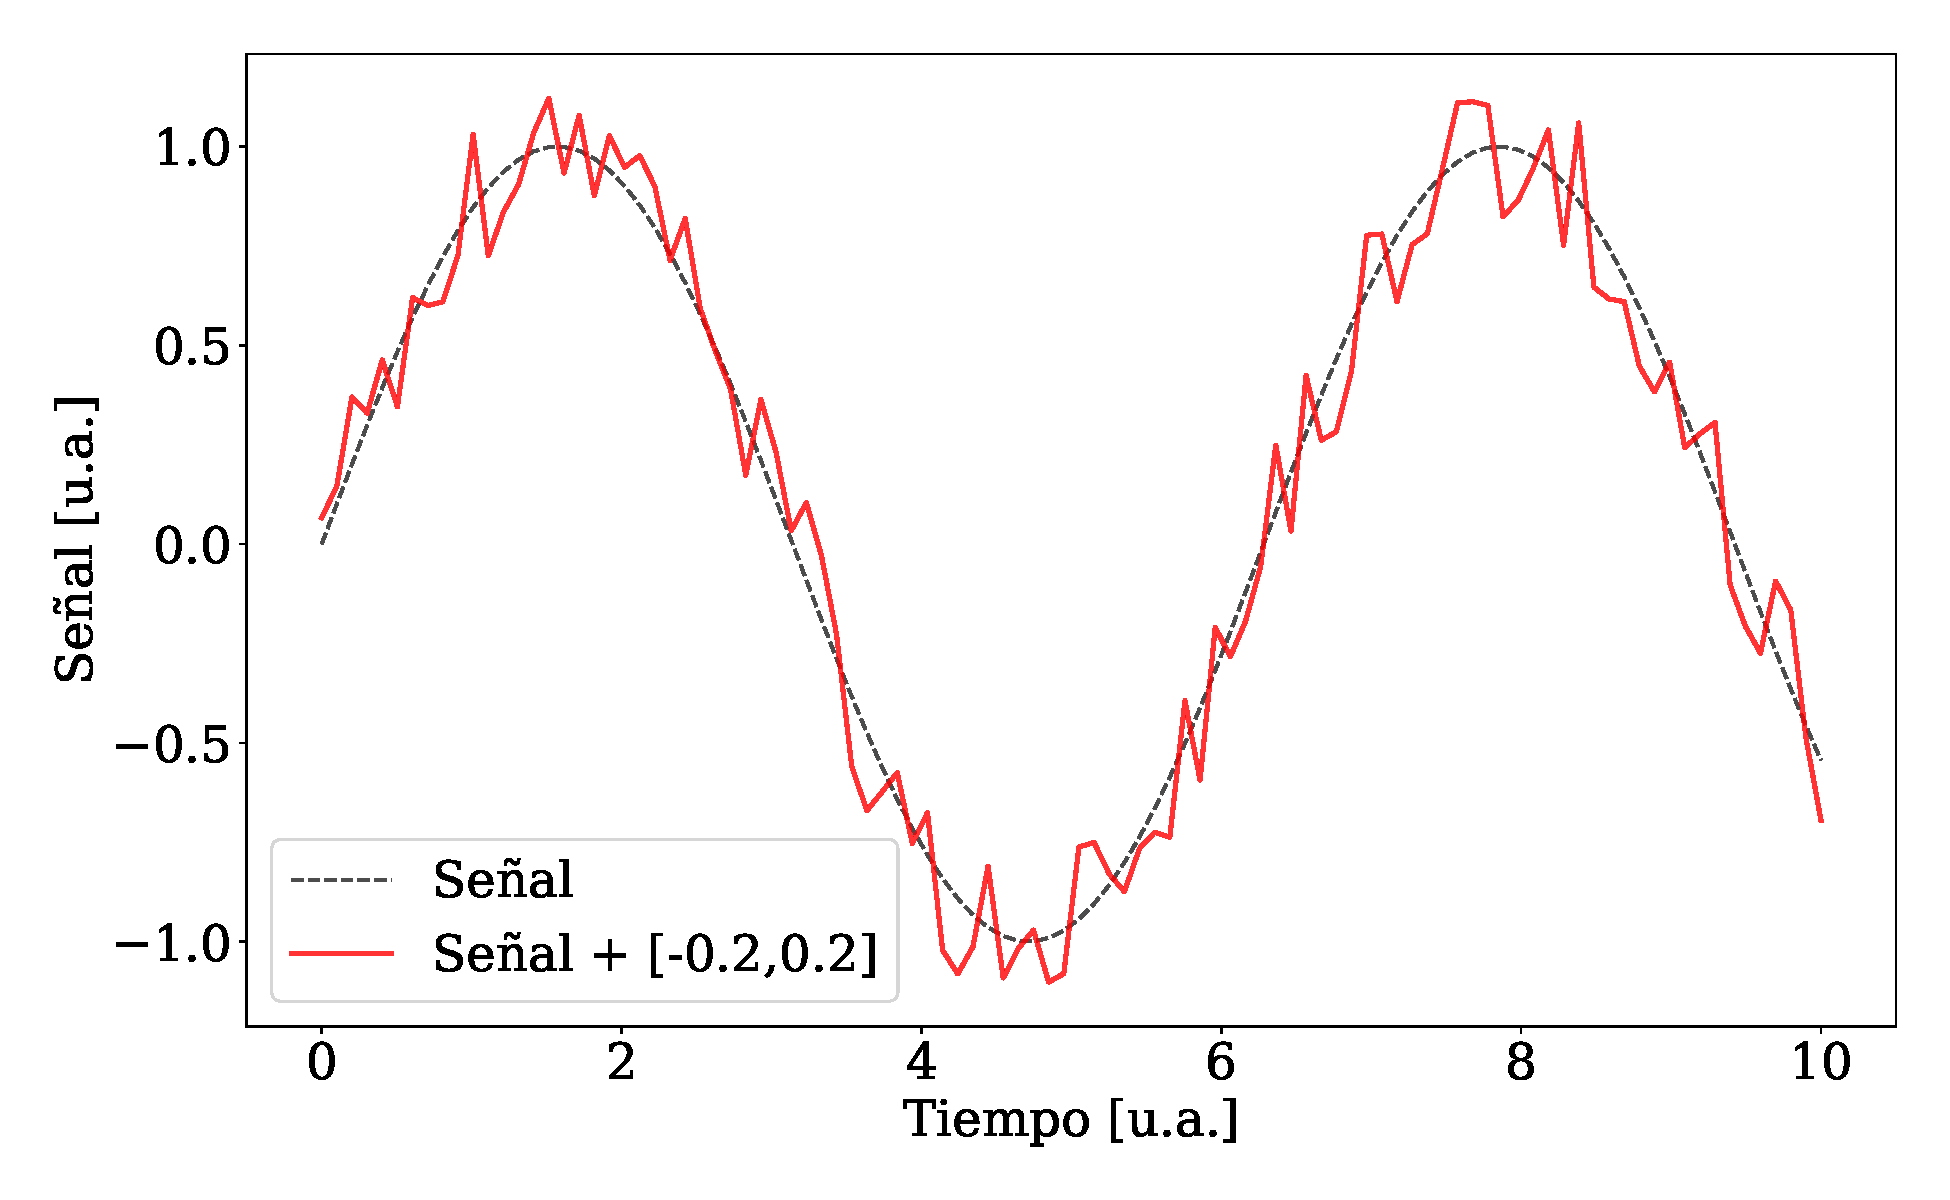
\includegraphics[width=0.5\textwidth]{ejer_15.pdf}
	\caption{Ejercicio 15}
	\label{fig:ejer15}
\end{figure}
	

\end{document}